% Chapter 6: Application Studies

\chapter{Application Studies}
\label{ch:sixth} % For referencing the chapter elsewhere, use \autoref{ch:name}
\label{chapter:codeGeneration-evaluation}

In this chapter we present application studies evaluating the performance of the \OpenCL code generated from expressions composed of parallel patterns using our systematic approach presented in the previous chapter.
We first discuss our experimental setup used for the runtime experiments.
We will start our evaluation by looking at the parallel reduction example which we used throughout the previous chapter and compare the performance of the manually optimized \OpenCL implementations against the systematically generated code.
We will then investigate application examples from linear algebra, mathematical finance, and physics.
We will conclude the chapter with a brief study showing how the rewrite rules can be applied automatically and how effective such an automatic search strategy is for a simple application example.

For all applications we show the high-level and low-level expression as well as performance results comparing the generated \OpenCL code against manually tuned \OpenCL code.

\section{Experimental Setup}
We used three hardware platforms: an Nvidia GeForce GTX 480 \GPU, an AMD Radeon HD 7970 \GPU and a dual socket Intel Xeon E5530 server, with 8 cores in total.
We used the latest \OpenCL runtime from Nvidia (CUDA-SDK 5.5), AMD (AMD-APP 2.8.1) and Intel (XE 2013 R3).
The GPU drivers installed were 310.44 for Nvidia and 13.1 for AMD on our Linux system.

We use the profiling \APIs from \OpenCL and \CUDA to measure kernel execution time and the \textit{gettimeofday} function for the \CPU implementation.
We exclude the data transfer time to and from the \GPU in all runtime numbers reported in this chapter, as we want to focus on the quality of the generated \OpenCL kernel code.
We repeat each experiment 100 times and report median runtimes.



\section{Parallel Reduction}
In this section we evaluate the performance of three of the low-level expressions presented in \autoref{sec:deriving:reduce} which resemble corresponding \OpenCL code provided by Nvidia performing a parallel summation of an array discussed at the beginning of \autoref{chapter:codeGeneration}.
All these expressions have been systematically derived from the high-level expression for the parallel summation:
\begin{equation*}
  vecSum = \reduce\ (+)\ 0
\end{equation*}
The formal derivations are shown in \autoref{chapter:AppendixA}.

\begin{figure*}[t]
\captionsetup[subfigure]{justification=justified,singlelinecheck=false}

\begin{subfigure}[b]{\linewidth}
\vspace{.4em}
\begin{minipage}{.05\linewidth}
\caption{}
\label{fig:reduce:expr:1}
\end{minipage}
\hfill
\begin{minipage}{.9\linewidth}
\begin{lstlisting}[mathescape, basicstyle=\small\rmfamily]
$vecSum = \reduce \circ \join \circ \mapWorkgroup\ \big($
    $\join \circ \toGlobal\ (\mapLocal\ (\mapSeq\ \id)) \circ \splitN\ 1\ \circ$
    $\iterateN\ 7\ (\join \circ \mapLocal\ (\reduceSeq\ (+)\ 0) \circ \splitN\ 2)\ \circ$
    $\join \circ \toLocal\ (\mapLocal\ (\mapSeq\ \id)) \circ \splitN\ 1$
  $\big) \circ \splitN\ 128$
\end{lstlisting}
\end{minipage}
\end{subfigure}

\begin{subfigure}[b]{\linewidth}
\vspace{0em}
\begin{minipage}{.05\linewidth}
\caption{}
\label{fig:reduce:expr:2}
\end{minipage}
\hfill
\begin{minipage}{.9\linewidth}
\begin{lstlisting}[mathescape, basicstyle=\small\rmfamily]
$vecSum = \reduce \circ \join \circ \mapWorkgroup\ \big($
    $\join \circ \toGlobal\ (\mapLocal\ (\mapSeq\ \id)) \circ \splitN\ 1\ \circ$
    $\iterateN\ 7\ \big(\ \lambda\ xs\ .\ \join \circ \mapLocal\ (\reduceSeq\ (+)\ 0) \circ \splitN\ 2\ \circ$
                $\reorderStride\ ((size\ xs)/2)\ \$\ xs\ \big)\ \circ$
    $\join \circ \toLocal\ (\mapLocal\ (\reduceSeq\ (+)\ 0)) \circ \splitN\ 2\ \circ$
    $\reorderStride\ 128$
  $\big) \circ \splitN\ (2\times 128)$
\end{lstlisting}
\end{minipage}
\end{subfigure}

\begin{subfigure}[b]{\linewidth}
\vspace{0em}
\begin{minipage}{.05\linewidth}
\caption{}
\label{fig:reduce:expr:3}
\end{minipage}
\hfill
\begin{minipage}{.9\linewidth}
\begin{lstlisting}[mathescape, basicstyle=\small\rmfamily]
$vecSum = \reduce \circ \join \circ \mapWorkgroup\ \big($
    $\join \circ \toGlobal\ (\mapLocal\ (\mapSeq\ \id)) \circ \splitN\ 1\ \circ$
    $\join \circ \mapWarp\ \big($
      $\join \circ \mapLane\ (\reduceSeq\ (+)\ 0) \circ \splitN\ 2\ \circ \reorderStride\ 1\ \circ$
      $\join \circ \mapLane\ (\reduceSeq\ (+)\ 0) \circ \splitN\ 2\ \circ \reorderStride\ 2\ \circ$
      $\join \circ \mapLane\ (\reduceSeq\ (+)\ 0) \circ \splitN\ 2\ \circ \reorderStride\ 4\ \circ$
      $\join \circ \mapLane\ (\reduceSeq\ (+)\ 0) \circ \splitN\ 2\ \circ \reorderStride\ 8\ \circ$
      $\join \circ \mapLane\ (\reduceSeq\ (+)\ 0) \circ \splitN\ 2\ \circ \reorderStride\ 16\ \circ$
      $\join \circ \mapLane\ (\reduceSeq\ (+)\ 0) \circ \splitN\ 2\ \circ \reorderStride\ 32$
    $\big) \circ \splitN\ 64\ \circ$
    $\join \circ \mapLocal\ (\reduceSeq\ (+)\ 0) \circ \splitN\ 2\ \circ \reorderStride\ 64\ \circ$
    $\join \circ \toLocal\ (\mapLocal\ (\reduceSeq\ (+)\ 0))\ \circ$
    $\splitN\ (blockSize/128)\ \circ \reorderStride\ 128$
  $\big) \circ \splitN\ blockSize$
\end{lstlisting}
\end{minipage}
\end{subfigure}

\caption{Three low-level expressions implementing parallel reduction.}
\label{fig:reduce:expr}
\end{figure*}


\autoref{fig:reduce:expr} shows the three expressions we will use for our performance comparison.
The first (\autoref{fig:reduce:expr:1}) corresponds to the first unoptimized Nvidia implementation (\autoref{lst:reduce1}),
the second (\autoref{fig:reduce:expr:2}) corresponds to an implementation by Nvidia with some optimizations applied (\autoref{lst:reduce3}), and
the third (\autoref{fig:reduce:expr:3}) corresponds to the fully optimized Nvidia implementation (\autoref{lst:reduce6}).


\begin{figure}
  \centering
  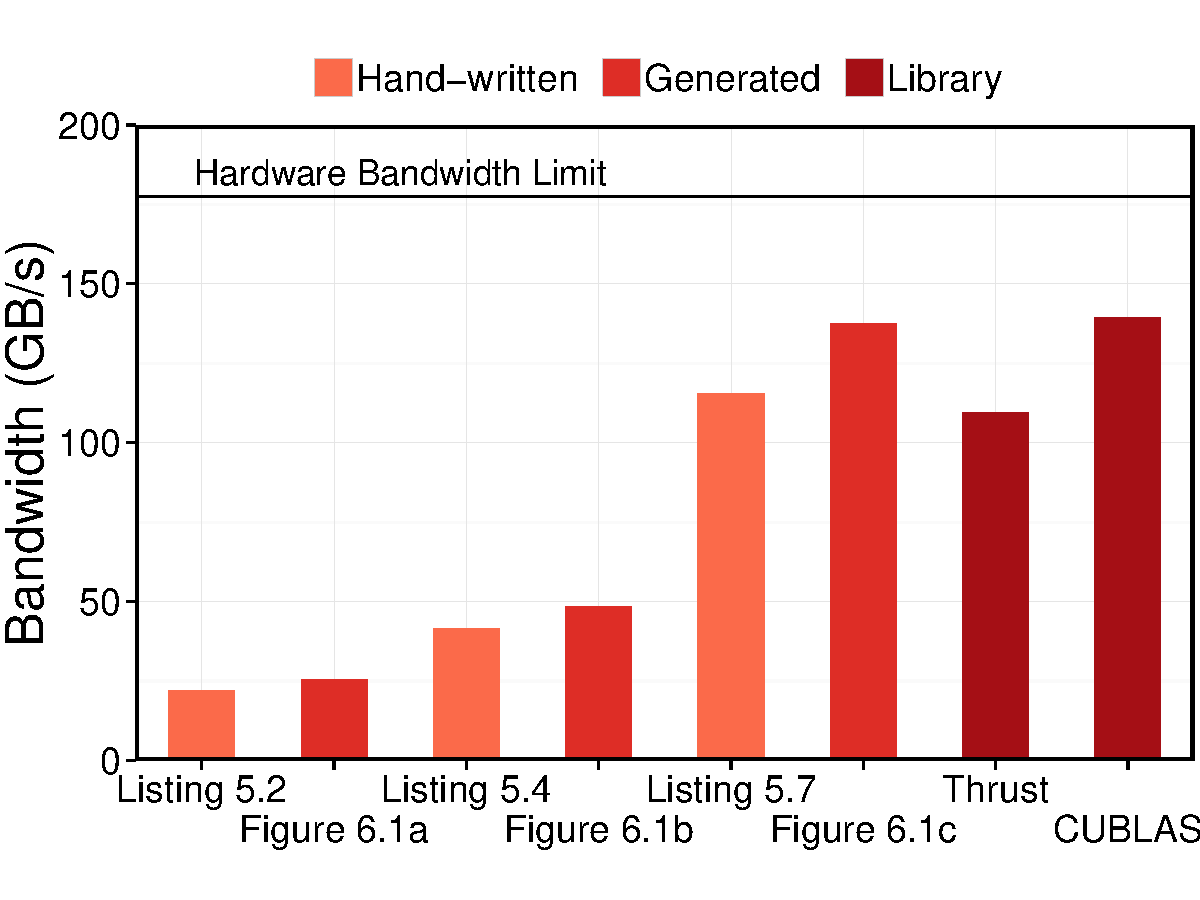
\includegraphics[width=.8\linewidth]{Plots/ReductionGenerator/reduce_runtime.pdf}
  \caption{Performance comparisons for code generated for three low-level expressions against native \OpenCL code.}
  \label{fig:reduce:expr:performance}
\end{figure}

\autoref{fig:reduce:expr:performance} shows the performance of these three versions compared to the corresponding native \OpenCL implementations by Nvidia and two additional libraries providing implementations of parallel reduction on \GPUs.
CUBLAS~\cite{cuBLAS} represents the CUDA-specific implementation of BLAS that only runs on Nvidia hardware.
Here we used the \emph{asum} benchmark for our comparison which performs a parallel reduction but first applies a function computing the absolute value on every element of the input vector.
We also include a parallel reduction implemented with Thrust~\cite{BellHo2011}, a library for simplified \GPU programming developed by Nvidia and based on \CUDA.

The results are reported as the achieved memory bandwidth which is computed from the absolute runtime of each version and the input data size.
This metric allows to compare each version against the hardware bandwidth limit.
The performance of the generated \OpenCL code from our three expressions matches, or even slightly outperforms, the corresponding native \OpenCL implementations written by Nvidia.
These results give some evidence that our systematically generated code can offer high performance, once the right set of optimizations -- encoded in our rewrite rules -- are applied.
The performance of our generated code for the fully optimized low-level expression even matches the performance of the highly optimized CUBLAS library written by Nvidia and outperforms the Thrust library.





\subsection{Automatically applying of the rewrite rules}

For the parallel reduction benchmark we implemented a prototype search tool automatically applying the rewrite rules for finding low-level expressions which offer high-performance.
Our prototype implementation starts with the high-level expression $\reduce\ (+)\ 0$ and transforms the expression using the rewrite rules and performs runtime experiments with the transformed expressions until a low-level \OpenCL expression is found which meats our performance expectations.
As discussed earlier in \autoref{chapter:codeGeneration} multiple rules might be valid to be applied for a given expression, therefore, we implemented a simple strategy for deciding which rules to apply.
This simple search strategy is loosely based on Bandit-based optimization~\cite{}.

Our search is an iterative process.
Given an expression we list all the rewrite rules which are valid to be applied.
We use a Monte Carlo method for evaluating the potential impact of each rule by randomly walking down the search tree.
We execute the code generated from the randomly chosen expressions and measure its performance.
The rule that promises the best performance following the Monte Carlo descent is chosen and the expression after the rule has been applied is used as the starting point for the next iteration.

This process is repeated until we reach an expression where there are no rules to be applied to.
In addition for selecting the rules, we also search at the same time for parameters controlling our primitives such as the parameter for the $\splitN\ n$ pattern.
We have limited the choices for these numerical parameters to a reasonable set of appropriate values for our test hardware.

We envision to replace this simplistic search strategy with more advanced techniques in the future.

\paragraph{Found expressions}
We performed the automatic search on all three of our hardware platforms.

\begin{figure*}[t]
\captionsetup[subfigure]{justification=justified,singlelinecheck=false}

\begin{subfigure}[b]{\linewidth}
\vspace{.4em}
\begin{minipage}{.15\linewidth}
\caption{Nvidia}
\label{fig:reduce:expr:auto:1}
\end{minipage}
\hfill
\begin{minipage}{.8\linewidth}
\begin{lstlisting}[mathescape, basicstyle=\small\rmfamily]
$\reduce \circ \join \circ \join \circ \mapWorkgroup\ \big($
   $\toGlobal\ (\mapLocal\ (\reduceSeq\ (+)\ 0))\circ \reorderStride\ 2048$
  $\big) \circ \splitN\ 128 \circ \splitN\ 2048$
\end{lstlisting}
\end{minipage}
\end{subfigure}

\begin{subfigure}[b]{\linewidth}
\vspace{0em}
\begin{minipage}{.15\linewidth}
\caption{AMD}
\label{fig:reduce:expr:auto:2}
\end{minipage}
\hfill
\begin{minipage}{.8\linewidth}
\begin{lstlisting}[mathescape, basicstyle=\small\rmfamily]
$\reduce \circ \join \circ \asScalar \circ \join \circ \mapWorkgroup\ \big($
    $\mapLocal\ \big(\mapSeq\ (\vect\ 2\ id) \circ$
      $\reduceSeq\ (\vect\ 2\ (+)\ 0)$
    $\big) \circ \reorderStride\ 2048$
  $\big) \circ \splitN\ 128\ \circ \asVector\ 2\ \circ \splitN\ 4096$
\end{lstlisting}
\end{minipage}
\end{subfigure}

\begin{subfigure}[b]{\linewidth}
\vspace{0em}
\begin{minipage}{.15\linewidth}
\caption{Intel}
\label{fig:reduce:expr:auto:3}
\end{minipage}
\hfill
\begin{minipage}{.8\linewidth}
\begin{lstlisting}[mathescape, basicstyle=\small\rmfamily]
$\reduce \circ \join \circ \mapWorkgroup\ \big( \join \circ \asScalar \circ \mapLocal($
    $\mapSeq\ (\vect\ 4\ id) \circ \reduceSeq\ (\vect\ 4\ (+))\ 0$
  $)\circ \asVector\ 4 \circ \splitN\ 32768\big) \circ \splitN\ 32768$
\end{lstlisting}
\end{minipage}
\end{subfigure}

\caption{Low-level expressions performing parallel reduction. These expressions are automatically derived by our prototype search tool from the  high-level expression $\reduce\ (+)\ 0$.}
\label{fig:reduce:expr:auto}
\end{figure*}

Figure~\ref{fig:reduce:expr:auto} shows the best performing low-level expression found by applying our automatic search technique.
The first expression (\autoref{fig:reduce:expr:auto:1}) was found on the Nvidia platform, the second (\autoref{fig:reduce:expr:auto:2}) on the AMD platform, and the third (\autoref{fig:reduce:expr:auto:3}) on the Intel platform.
We can make several important observations.
The first observation is, that none of the expressions make use of the local memory (although our systems fully support it).
It is common wisdom that using local memory on the \GPU enables high performance and in fact the highly tuned hand-written implementation of \textit{asum} use local memory on the \GPU.
However, as we will see later in the results section, our automatically derived version is able to perform as well without using local memory.
The second key observation is, that each work-item performs a large sequential reduction independent of all other threads, which does not require synchronization and, thus, avoids overheads.

While these observations are the same for all platforms, there are also crucial differences between the different low-level expressions.
Both \GPU expressions make use of the \reorderStride primitive, allowing for coalesced memory accesses.
The AMD and Intel expressions are vectorized with a vector length of two and four respectively.
The Nvidia version does not use vectorization since this platform does not benefit from vectorized code.
On the \CPU, the automatic search picked numbers for partitioning into work-groups and then into work-items in such a way that inside each work-group only a single work-item is active.
This reflects the fact that there is less parallelism available on a \CPU compared to \GPUs.

Interestingly, the results of our search have some artifacts in the expressions.
For example, we perform unnecessary copies on AMD and Intel by performing a \mapSeq with the identity nested inside.
While this does not seem to affect performance much, a better search strategy could probably get rid of these artifacts and might achieve a slightly better performance.


\paragraph{Performance of found expressions}
\autoref{fig:reduce:expr:automatic:performance} shows the performance of the code generated for the three expressions shown in \autoref{fig:reduce:expr:auto} performing a parallel reduction compared against the highly tuned implementations of \emph{asum}.
The three plots show the performance for the Nvidia platform (on the left), the AMD platform (in the middle), and the Intel platform (on the right).
All plots are scaled according to the hardware bandwidth limit of the platform.
On each platform we compare against a vendor provided, highly tuned implementation of the BLAS library, where we measured the bandwidth achieved for the \emph{asum} application.
Where in the \emph{asum} application an additional operation (applying the absolute value function) is performed for every data item, we showed in \autoref{section:skelcl:evaluation:linearAlgebra} that the performance difference for the parallel reduction benchmark and the \emph{asum} benchmark is negligible when both are implemented properly.
Therefore, we consider the BLAS implementations as a valid contender for a fair performance comparison.

\begin{figure}
  \centering
  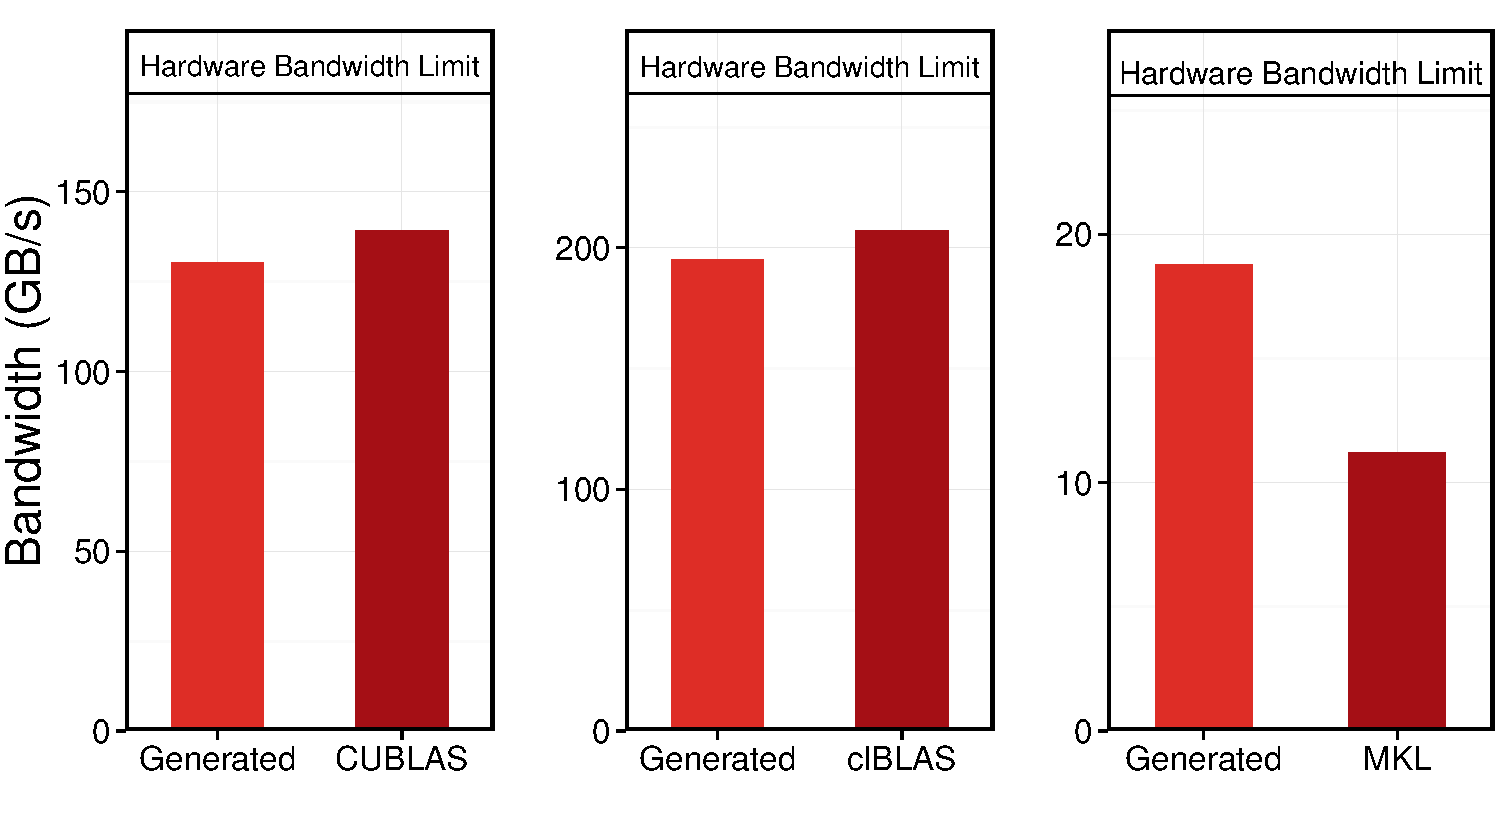
\includegraphics[width=\linewidth]{Plots/ReductionGenerator/reduce_automatic_runtime.pdf}
  \caption{Performance comparisons for code generated for three automatically found low-level expressions against hardware-specific library code on three platforms.}
  \label{fig:reduce:expr:automatic:performance}
\end{figure}

The results shows that the generated code for the automatically found expressions are on par with the CUBLAS implementation of Nvidia and the clBLAS implementation of AMD achieving about 95\% of their performance.
On the Intel platform our generated code actually outperforms the MKL implementation.
This is due to the implementation of MKL and the particular multi-core \CPU used.
For the \emph{asum} benchmark the MKL implementation does not use thread level parallelism, presumably with the assumption that \emph{asum} is a memory bound benchmark.
The used multi-core \CPU is actually a two socket machine where two chips are combined on a single motherboard.
In this configuration there are two memory controllers available -- one for each socket.
Therefore, thread level parallelism is actual beneficial for the \emph{asum} benchmark on this particular hardware giving our generated code a speedup of 1.67.

The three plots together also show that our approach offers true performance portability.
Where each BLAS implementation is not-portable and bound to a specific hardware architecture, our system automatically searched and found three expressions systematically derived from a single high-level representation which offer high performance on all three platforms.
With our approach we achieve the same relative performance on all platforms which is within 75\% of the corresponding hardware bandwidth limit.


\paragraph{Search Efficiency}
We now investigate the efficiency of our simple search strategy.
Figure~\ref{fig:search} shows how many expressions were evaluated during the search.
The evaluated expressions are grouped from left to right by the number of rules applied in the search tree.
The red line connects the fastest expression found so far.

\begin{figure*}[t]
%
\begin{subfigure}[b]{0.48\linewidth}
\includegraphics[width=\linewidth]{nv\string_search.pdf}
\caption{Nvidia GPU}
\label{fig:search:nv}
\end{subfigure}
\hfill
%
\begin{subfigure}[b]{0.48\linewidth}
\includegraphics[width=\linewidth]{amd\string_search.pdf}
\caption{AMD GPU}
\label{fig:search:amd}
\end{subfigure}
\\
\centering
%
\begin{subfigure}[b]{0.48\linewidth}
\includegraphics[width=\linewidth]{intel\string_search.pdf}
\caption{Intel CPU}
\label{fig:search:intel}
\end{subfigure}

\caption{
   Search efficiency.
   The vertical partitioning represents the number of fixed derivations in the search tree.
   The red line connects the fastest expressions found so far.
}
\label{fig:search}
\end{figure*}

As can be seen the performance improves steadily for all three platforms before reaching a plateau.
For both \GPUs the best performance is reached after testing about 40 expressions.
At this point we have fixed five derivations and found a subtree offering good performance for some expressions.
Nevertheless, even in the later stages of the search many expressions offer bad performance, which is partly due to the sensitivity of \GPU for selecting appropriate numerical parameters.
On the \CPU performance converges quicker and more expressions offer good performance.
This shows that the \CPU is easier to optimize for and not as sensitive when selecting numerical parameters.

\bigskip

\noindent
This results show, that applying our rules automatically is feasible and capable of finding high performing low-level expressions for high-level expressions written by the programmer.
Our approach offers true performance portability where the portable high-level expression is systematically and automatically optimized for a particular hardware architecture delivering similar relative performance on all tested devices.
Nevertheless, we only tested our simple automatic search strategy with the parallel reduction benchmark.
For more complex applications the search space becomes bigger and possible more advanced search techniques have to be applied.
We intend to work on this topic more in the future, as we will discuss in more detail in \autoref{section:future-work}.


\section{Linear Algebra Applications}

For our linear algebra benchmarks, we have performed experiments with multiple input sizes.
For \bench{scal}, \bench{asum} and \bench{dot}, the small input size corresponds to a vector size of 16M elements (64MB).
The large input size uses 128M elements (512MB, the maximum OpenCL buffer size for our platforms).
For \bench{gemv}, we use an input matrix of 4096$\times$4096 elements (64MB) and a vector size of 4096 elements (16KB) for the small input size.
For the large input size, the matrix size is 8192$\times$16384 elements (512MB) and the vector size 8192 elements (32KB).


We choose linear algebra kernels as our first set of benchmarks, because they are well known, easy to understand, and used as building blocks in many other applications.
Figure~\ref{lst:linear-algebra-expr} shows how we express vector scaling, sum of absolute values, dot product of two vectors and matrix vector multiplication using our high-level patterns.
While three benchmarks perform computations on vectors, matrix vector multiplication illustrates a computation using a 2D data structures.

For scaling (line~5), the \pat{map} pattern applies a function to each element which multiplies it with a constant.
This function is expressed by partially applying the \code{mult} function, \ie binding \code{a} to the first argument of \code{mult}.
The sum of absolute values (line~6) and the dot product (line~7) applications both produce scalar results by performing a summation, which we express using the \pat{reduce} pattern combined with the addition.
For dot product, a pair-wise multiplication of its two input vectors is performed before applying the reduction.
This is expressed using the \pat{zip} and \pat{map} patterns.

Line~8--10 shows matrix vector multiplication as defined in BLAS: $\vec{y} = \alpha A \vec{x} + \beta \vec{y}$.
To multiply $A$ with $\vec{x}$, the \pat{map} pattern maps the computation of the dot-product with the input vector $\vec{x}$ to each row of the matrix $A$ (line~9).
Notice how we are reusing the high-level expressions for dot-product. % and scaling as building blocks for the more complex matrix-vector multiplication.
This shows the power of our system: expressions describing algorithmic concepts can be reused, without committing to a particular low-level implementation.
The dot-product from gemv (line~9) might be implemented in a totally different way from the stand-alone dot-product.

\begin{lstlisting}[%
  float,%
  caption={Linear algebra kernels from the BLAS library expressed using our high-level algorithmic patterns.},%
  label={lst:linear-algebra-expr}%
  ]
add x y  = x + y
mult x y = x * y
abs x    = if (x < 0) -x else x

scal a xs = map (mult a) xs
asum xs   = reduce add 0 (map abs xs)
dot xs ys = reduce add 0 (map mult (zip xs ys))

gemv A xs ys a b =
  map (
    \ (Ar, y) ->
      map add (zip
        (scal a $\circ$ dot xs Ar)
        scal b y
      )
  ) (zip A ys)
\end{lstlisting}


\subsection{Comparison vs. Portable Implementation}
% OpenCL is not performance portable

\begin{figure}[t]
  \includegraphics[width=\linewidth]{PLDI2015/application\string_results\string_vs\string_clBLAS}
  \caption{Performance of our approach relative to a portable OpenCL reference implementation (clBLAS).
           We outperform it on most benchmarks and platforms.}
  \label{fig:clblas}
\end{figure}

First, we show how our approach performs across three platforms.
We use the BLAS OpenCL implementations written by AMD as our baseline for this evaluation since it is inherently portable across all different platforms.
Figure~\ref{fig:clblas} shows the performance of our approach relative to clBLAS for the BLAS routines.
As can be seen, we achieve better performance than clBLAS on most platforms and benchmarks.
The speedups are the highest for the CPU, with up to 20$\times$ for the \bench{asum} benchmark with a small input size.
The reason is that clBLAS was written and tuned specifically for an AMD GPU which usually exhibit a larger number of parallel processing units.
As we saw in Section~\ref{search}, our systematically derived expression for this benchmark is specifically tuned for the CPU by avoiding creating too much parallelism, which is what gives us such large speedup.

Figure~\ref{fig:clblas} also shows the results we obtain relative to the Nvidia SDK \bench{BlackScholes} and SHOC molecular dynamics \bench{MD} benchmark.
For \bench{BlackScholes}, we see that our approach is on par with the performance of the Nvidia implementation on both GPUs.
On the CPU, we actually achieve a 2.2$\times$ speedup due to the fact that the Nvidia implementation is tuned for GPUs while our implementation generates different code for the CPU.
For \bench{MD}, we are actually on par with the OpenCL implementation on all platforms.

\subsection{Comparison vs. Highly-tuned Implementations}

\begin{figure*}[t]
  \centering
  \begin{subfigure}[b]{0.315\linewidth}
    \includegraphics[width=\linewidth]{PLDI2015/application\string_results\string_vs\string_BEST\string_nv}
    \caption{Nvidia GPU}
    \label{fig:results-nv}
  \end{subfigure}
  \hspace{0.015\linewidth}
  \begin{subfigure}[b]{0.315\linewidth}
    \includegraphics[width=\linewidth]{PLDI2015/application\string_results\string_vs\string_BEST\string_amd}
    \caption{AMD GPU}
    \label{fig:results-amd}
  \end{subfigure}
  \hspace{0.015\linewidth}
  \begin{subfigure}[b]{0.315\linewidth}
    \includegraphics[width=\linewidth]{PLDI2015/application\string_results\string_vs\string_MKL\string_intel}
    \caption{Intel CPU}
    \label{fig:results-cpu}
  \end{subfigure}
  \vspace{-1.5em}
  \caption{Performance comparison with state of the art platform-specific libraries; CUBLAS for Nvidia, clBLAS for AMD, MKL for Intel.
           Our approach matches the performance on all three platforms and outperforms clBLAS in some cases.
           %of CUBLAS and MKL, and outperforms clBLAS on some routines.
         }
   \label{fig:results}
\end{figure*}

We compare our approach with a state of the art implementation for each platform.
For Nvidia, we pick the highly tuned CUBLAS implementation of BLAS written by Nvidia.
For the AMD GPU, we use the same clBLAS implementation as before given that it has been written and tuned specifically for AMD GPUs.
Finally, for the CPU we use the Math Kernel Library (MKL) implementation of BLAS written by Intel, which is known for its high performance.

Figure~\ref{fig:results-nv} shows that we actually match the performance of CUBLAS for \bench{scal}, \bench{asum} and \bench{dot} on the Nvidia GPU.
For \bench{gemv} we outperform CUBLAS on the small size by 20\% while we are within 5\% for the large input size.
Given that CUBLAS is a proprietary library highly tuned for Nvidia GPUs, these results should offer some confidence that our technique is able to achieve high performance.

On the AMD GPU, we are surprisingly up to 4.5$\times$ faster than the clBLAS implementation on \bench{gemv} small input size as shown in Figure~\ref{fig:results-amd}.
The reason for this is found in the way clBLAS is implemented.
%For the \bench{gemv} benchmark,
clBLAS performs automatic code generation using fixed templates.
In contrast to our approach, they only generate one implementation since they do not explore different pattern compositions.

For the Intel CPU (Figure~\ref{fig:results-cpu}), our approach beats MKL for one benchmark and matches the performance of MKL on most of the other three benchmarks.
For the small input sizes for the \bench{scal} and \bench{dot} benchmarks we are within 13\% and 30\% respectively.
For the larger input sizes, we are on par with MKL for both benchmarks.
The \bench{asum} implementation in the MKL does not use thread level parallelism, where our implementation does and, thus, achieves a speedup of up to 1.78 on the larger input size.


This section has shown that our approach generates \emph{performance portable} code which is competitive with highly-tuned platform specific implementations.










\section{Mathematical Finance}

For \bench{BlackScholes}, the problem size is fixed to 4 million elements and for \bench{MD} it is 12288 particles.

The BlackScholes application uses a Monte-Carlo method for option pricing and computes for each stock price \code{s} a pair of call and put options \code{\{c,p\}}.
Figure~\ref{fig:blackScholes} shows the BlackScholes implementation, where the function defined in line~1 computes the call and put option for a single stock price \code{s}.
Two intermediate results \code{d1} and \code{d2} are computed and used to compute the two options, which are returned as a single pair.
% The \code{compD1}, \code{compD2}, \code{compCall} and \code{compPut} functions are not shown here since they only contain purely sequential code implementing the BlackScholes model.
This \code{BSComputation} function is applied to all stock prices, stored in a vector $\vec{s}$, using the \pat{map} pattern in line~4.


\begin{lstlisting}[%
  float,%
  caption={BlackScholes mathematical finance application expressed using our high-level algorithmic patterns.},%
  label={lst:bs-expr}%
  ]
BSComputation s =
  d1 = compD1 s
  d2 = compD2 d1 s
  { compCall d1 d2 s, compPut d1 d2 s }

blackScholes = map BSComputation
\end{lstlisting}
\begin{figure}[t]
  \includegraphics[width=\linewidth]{PLDI2015/application\string_results\string_vs\string_clBLAS}
  \caption{Performance of our approach relative to a portable OpenCL reference implementation (clBLAS).
           We outperform it on most benchmarks and platforms.}
  \label{fig:clblas}
\end{figure}














\section{Physics Application}

For \bench{BlackScholes}, the problem size is fixed to 4 million elements and for \bench{MD} it is 12288 particles.


Another application we consider is the molecular dynamics (MD) application from the SHOC~\cite{danalis10shoc} benchmark suite.
It calculates the sum of all forces acting on a particle from its neighbors.
Figure~\ref{fig:md} shows the implementation using our high-level patterns.

The function \code{updateF} (line~1) updates the force \code{f} of particle \code{p} by computing and adding the force between a single particle and one of its neighbors.
%\code{updateF} takes an index of a neighbor \code{nId}, the vector storing all particles $\vec{p}$, and a threshold \code{t} as additional parameters.
Using the neighbor's index \code{nId} and the vector storing all particles $\vec{p}$ the neighboring particle is accessed and the distance is computed (line~2).
%between the neighboring particle and the particle \code{p} ist computed.
If the distance is below threshold \code{t} the force between the two particles is calculated and added to the overall force \code{f} (line~3).
% Otherwise the particle is ignored in the summation.



%
%


For computing the force for all particles $\vec{p}$, we use the \pat{zip} pattern~(line~7) to build a vector of pairs, where each pair combines a single particle with the indices of all of its neighboring particles.
The function which is applied to each pair by the \pat{map} pattern~(line~5) is expressed as an lambda expression~(line~6).
Computing the resulting force exerted by all the neighbors on one particle is done by applying the \pat{reduce} pattern on vector $\vec{n}$ storing the neighboring indices.
We use function \code{updateF} inside the reduction to compute the force for each particle with index \code{nId} and add it to the overall force on \code{p}.
% At this point we fix all but the first two arguments as the other arguments remain constant for particle \code{p}.
The usage of lambda expressions in our system allows for easy binding of additional information as arguments to functions.
This application example should give some evidence that our patterns are flexible enough to implement real world applications.


\begin{lstlisting}[%
  float,%
  caption={Molecular dynamics physics application expressed using our high-level algorithmic patterns.},%
  label={lst:md-expr}%
  ]
updateF f nId p ps t =
  n = ps[nId]
  d = calculateDistance p n
  if (d < t) f + (calculateForce d)
  else       f

md ps N t = map (
    $\lambda$ (p, ns) $\rightarrow$
      reduce ($\lambda$ (f, nId) $\rightarrow$ updateF f nId p ps t) 0 ns
  ) (zip ps N)
\end{lstlisting}

\begin{figure}[t]
  \includegraphics[width=\linewidth]{PLDI2015/application\string_results\string_vs\string_clBLAS}
  \caption{Performance of our approach relative to a portable OpenCL reference implementation (clBLAS).
           We outperform it on most benchmarks and platforms.}
  \label{fig:clblas}
\end{figure}



%\from{PACT begin}
%This section presents the applications we have used to evaluate our approach.
%We discuss how applications from linear algebra, physics, and mathematical finance can be represented as expressions composed of our high-level algorithmic patterns.
%Furthermore, we discuss how our rules are used to systematically rewrite and optimize expressions.
%\from{PACT end}
%
%\from{PACT begin}
%\section{Experimental Setup (PACT)}
%\subsection{Platform and Performance Measurement}
%
%We used three hardware platforms to perform the experiments: an Nvidia GeForce GTX 480 GPU, an AMD Radeon HD 7970 GPU and a dual socket Intel Xeon E5530 server, with 8 cores in total and hyper-threading enabled.
%We used the latest OpenCL runtime from Nvidia (CUDA-SDK 5.5), AMD (AMD-APP 2.8.1) and Intel (XE 2013 R3 3.2.1.16712).
%The GPU drivers installed on our Linux system were 310.44 for Nvidia and 13.1 for AMD.
%ATLAS is built as an auto-tuned multi-threaded C library using gcc 4.7.2.
%
%We use the profiling function from the OpenCL and CUDA API to measure kernel execution time and the \textit{gettimeofday} function in the case of the ATLAS implementation.
%Following the Nvidia benchmarking methodology~\cite{Harris07reduction}, the data transfer time to and from the GPU is excluded.
%We repeat each experiment 1000 times and report the median runtime.
%
%\subsection{Input Sizes}
%
%For our linear algebra benchmarks, we have performed experiments with two input sizes.
%For \bench{scal}, \bench{asum} and \bench{dot}, the small input size corresponds to a vector size of 16M elements which translates to 64MB of data.
%The large input size uses 128M elements which correspond to 512MB (the maximum OpenCL buffer size for our platforms).
%
%For \bench{gemv}, we use an input matrix of 4096 $\times$ 4096 elements (64MB) and a vector size of 4096 elements (16KB) for the small input size.
%For the large input size, the matrix size is 8192 $\times$ 16384 elements (512MB) and the vector size 8192 elements (32KB).
%For \bench{BlackScholes}, the problem size is fixed to 4 million elements and for \bench{MD} it is 12288 particles.
%
%\subsection{Benchmarks}
%
%\begin{table*}[t]
%\centering
%\renewcommand{\arraystretch}{1.25}
%\rowcolors{2}{oddcolor}{evencolor}
%\setlength{\tabcolsep}{3pt}
% \begin{tabular}{lrclrcl}
%  \toprule
%  \tabhead{Name} & \multicolumn{3}{c}{\tabhead{Formula}} & & & \multicolumn{1}{l}{\tabhead{High-level expression}}\\
%  \midrule
%  Vector scale & $\vec{x}$&$=$&$\alpha \vec{x}$
%               & $scal(\alpha, \vec{x})$&$=$&$map(\ast \alpha,\ \vec{x})$\\
%  Sum of abs. values & $c$&$=$&$\sum_i |x_i|$
%                   & $asum(\vec{x})$&$=$&$reduce(+,0) \circ map(abs,\ \vec{x})$\\
%  Dot product & $c$&$=$&$\sum_i (x_i \ast y_i) $
%                & $dot(\vec{x}, \vec{y})$&$=$&$reduce(+,0) \circ map(\ast) \circ zip(\vec{x},\ \vec{y})$\\
%  \rule{0pt}{13pt}% make the row higher at the top ...
%  Matrix-vector mult. & $\vec{y}$&$=$&$\alpha A\vec{x} + \beta \vec{y}$
%                      & \hspace{.2em}$ gemv(A, \vec{x}, \vec{y}, \alpha, \beta)
%                          $&$=$&$map(+) \circ zip\Big(
%                          map\big(scal(\alpha) \circ dot(\vec{x}) ,\ A\big),\
%                      scal(\beta, \vec{y})\Big) $\\[.25em]% ... and the bottom
%  BlackScholes & $ \langle\vec{c}, \vec{p}\rangle$&$=$&$\text{\textit{BSModel}}(\vec{s}) $ & $\text{\textit{BlackScholes}}(\vec{s})$&=&$map(\text{\textit{BSModel}},\ \vec{s})$\\
%  Molecular Dyn. (MD)           & &&& \multicolumn{3}{c}{$map\big(reduce(\text{\textit{calculateForce}}, 0)\big) \circ zip(\text{\textit{particles}}, \text{\textit{neighArray}})$}\\
%  \bottomrule
% \end{tabular}
%\caption{Benchmarks used for our experiments.}
%\label{tab:benchmarks}
%\end{table*}
%
%Our list of benchmarks is shown in Table~\ref{tab:benchmarks} with the corresponding high-level expression written by the programmer.
%The first three benchmarks perform well-known computations on 1D vectors of floats: scaling, computing the sum of absolute values, and computing the dot product of two vectors.
%For scaling, the \pat{map} pattern combined with the $\ast\alpha$ function multiplies every element of the vector with the constant $\alpha$.
%The sum of absolute values and the dot product applications both produce scalar results by performing a summation, which we express using the \pat{reduce} pattern combined with the addition.
%Before performing the reduction in the dot product application a pair-wise multiplication of its two input vectors is performed.
%This is expressed using the \pat{zip} and \pat{map} patterns.
%
%Matrix vector multiplication was chosen to illustrate a case where we perform computation on a 2D data structure.
%The expression in the fourth row of Table~\ref{tab:benchmarks} describes this benchmark.
%The \pat{map} nested inside the \pat{zip} maps the computation of the dot-product with the input vector $\vec{x}$ to each row of the matrix $A$.
%Notice how we are reusing the high-level expressions for dot-product and scaling a vector as basic building blocks for the more complex matrix-vector multiplication.
%This shows the power of our system where expressions describing concepts at the algorithmic level can be reused, without committing to a particular low-level implementation.
%
%Finally, we want to show that our technique is not limited to linear algebra and can be applied to any benchmark that can be express in terms of our high-level patterns.
%BlackScholes uses a Monte-Carlo method for option pricing and MD, from SHOC~\cite{danalis10shoc}, calculates forces between particles.
%Table~\ref{tab:benchmarks} shows that BlackScholes can be easily expressed with a \pat{map} pattern since this problem is embarrassingly parallel: for each stock price $s_i$ the BlackScholes model computes a pair of call and put options $\langle c_i, p_i\rangle$.
%MD calculates the sum of all forces acting on each particles from their neighbors.
%The neighborArray represents an array of neighbors, with each row corresponding to the neighbors of a particular particle from the particles array.
%The reduction inside \pat{map} calculates the resulting force exercised on one particular particle by all neighbor particles.
%
%
%\subsection{Example: Sum of Absolute Values}
%\label{sec:example}
%
%This section shows our rules in action transforming an expression to compute the sum of the absolute values of a vector (the \emph{asum} benchmark from Table~\ref{tab:benchmarks}).
%The computation can easily be expressed using two of our high-level algorithmic patterns:
%$reduce(+, 0,\ map(abs,\ \vec{x}))$.
%First, the $abs$ function is applied to every element of the input vector $\vec{x}$ and then the intermediate result is summed up using the $reduce$ pattern which is customized with the plus operator.
%Using the function composition operator, we write this expression in a more functional style:
%$reduce(+, 0) \circ map(abs)$.
%This simplifies the reasoning about this expression as unnecessary details (e.g. the name of the input vector) are omitted.
%
%We are transforming this expression in several steps using our rules as shown in Figure~\ref{fig:derivation}.
%The letter/number combination for each rule refers to Figure~\ref{fig:algo} or~\ref{fig:low}.
%First, we apply the reduction rule to replace \pat{reduce} with \pat{reduce} $\circ$ \pat{part-red} and then immediately apply the same rule again to expand \pat{par-red}.
%The double application of rule~\ref{fig:algo:red} is shown as Step 1 in Figure~\ref{fig:derivation}.
%Afterwards, we expand the \pat{map} (Step 2), which allows us to simplify the expression by removing the two corresponding \pat{outerJoin} and \pat{outerSplit} patterns (Step 3).
%After fusing two \pat{maps} (Step 4), we lower the \pat{map} and \pat{reduce} patterns in Step 5.
%Finally, we apply rule~\ref{fig:algo:fusion} to fuse the \pat{map-seq} and \pat{reduce-seq} into a single \pat{reduce-seq} (Step 6).
%This sequence of transformations results in a more optimal implementation since no temporary storage is required for the intermediate result.
%
%This example shows how our system can systematically optimize programs at an algorithmic level without performing complex compiler analysis.
%
%\begin{figure}[t]
%\centering
%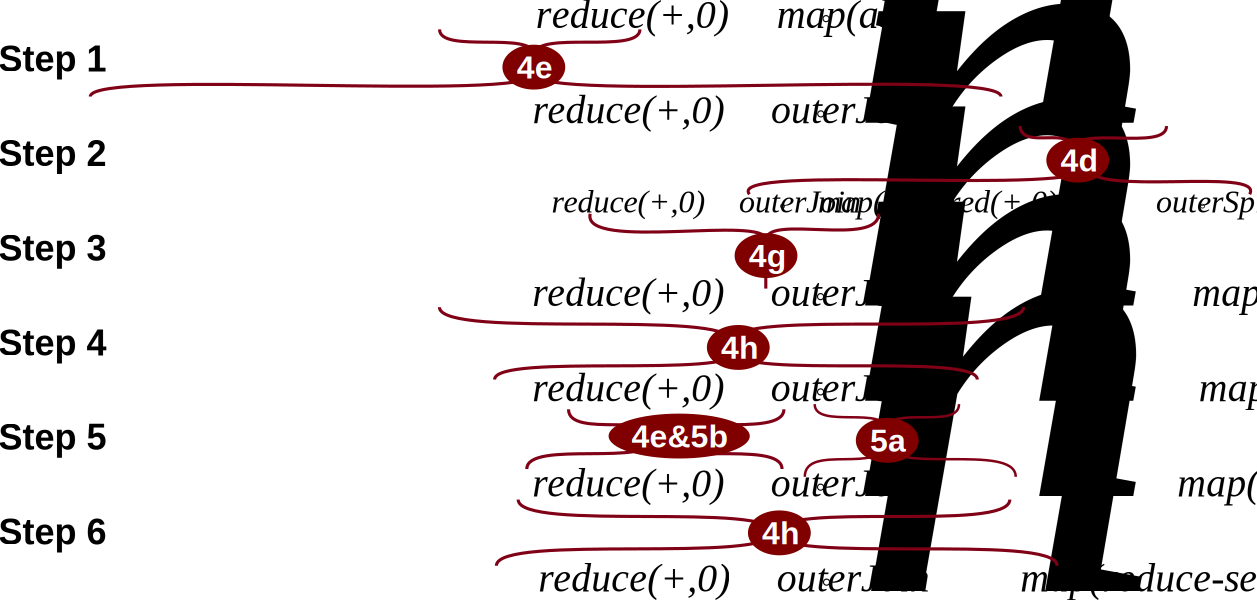
\includegraphics[width=\linewidth]{PACT2014/derivation4-times}
%\caption{Derivation for $asum(\vec{x})$ to a fused version.
%  The number in the circles refers to the used rule.
%}
%\label{fig:derivation}
%\end{figure}
%\from{PACT end}
%
%
%\section{Linear Algebra Applications}
%
%  \subsection{Level-1 BLAS Routines}
%
%    \paragraph{Vector scale}
%
%    \paragraph{Sum of absolute balues}
%
%    \paragraph{Dot product}
%
%  \subsection{Matrix-Vector Multiplication}
%
%\section{Mathematical Finance}
%
%\section{Physics Simulation}
%
%\from{PACT begin}
%\section{Experiments (PACT)}
%
%We now evaluate our approach compared to reference OpenCL implementations of our benchmarks on all platforms.
%Furthermore, we compare the BLAS routines against platform-specific tuned implementations.
%We also analyze the expression found automatically for one of our benchmarks.
%
%
%
%
%\subsection{Comparison vs. Portable Implementation}
%
%\begin{figure}[t]
%  \includegraphics[width=\linewidth]{PACT2014/application\string_results\string_vs\string_clBLAS}
%  \caption{Performance of our approach relative to a portable OpenCL reference implementation.
%           We outperform the clBLAS implementation on most benchmarks and platforms.}
%  \label{fig:clblas}
%\end{figure}
%
%We want to show how our approach performs across three platforms.
%We use the BLAS OpenCL implementations written by AMD as our baseline for this evaluation since it is inherently portable across our different platforms.
%Figure~\ref{fig:clblas} shows the performance of our approach relative to clBLAS~\cite{clBLAS} for the BLAS routines.
%As can be seen, we achieve better performance than clBLAS on most platforms and benchmarks.
%The speedups are the highest on the CPU, with up to 20$\times$ for the \bench{asum} benchmark with a small input size.
%The reason is that clBLAS was written and tuned specifically for an AMD GPU which usually exhibit a larger number of parallel processing units.
%As we will see later, our automatically derived expression for this benchmark is specifically tuned for the CPU by avoiding creating too much parallelism, which is what gives us such large speedup.
%
%Figure~\ref{fig:clblas} also shows the results we obtain relative to the Nvidia SDK \bench{BlackScholes} and SHOC molecular dynamics \bench{MD} benchmark.
%For \bench{BlackScholes}, we see that our approach is on par with the performance of the Nvidia implementation on both GPUs.
%On the CPU, we actually achieve a 2.2$\times$ speedup due to the fact that the Nvidia implementation is tuned for GPUs while our implementation generates different code for the CPU.
%For \bench{MD}, we are actually on par with the OpenCL implementation on all platforms.
%
%
%\subsection{Comparison vs. Highly-tuned Implementations}
%
%\begin{figure*}[t]
%  \centering
%  \begin{subfigure}[b]{0.315\linewidth}
%    \includegraphics[width=\linewidth]{PACT2014/application\string_results\string_vs\string_BEST\string_nv}
%    \caption{Nvidia GPU}
%    \label{fig:results-nv}
%  \end{subfigure}
%  \hfill
%  \begin{subfigure}[b]{0.315\linewidth}
%    \includegraphics[width=\linewidth]{PACT2014/application\string_results\string_vs\string_BEST\string_amd}
%    \caption{AMD GPU}
%    \label{fig:results-amd}
%  \end{subfigure}
%  \hfill
%  \begin{subfigure}[b]{0.315\linewidth}
%    \includegraphics[width=\linewidth]{PACT2014/application\string_results\string_vs\string_BEST\string_intel}
%    \caption{Intel CPU}
%    \label{fig:results-cpu}
%  \end{subfigure}
%  \caption{Performance comparison of our approach relative to a highly-tuned platform-specific library; CUBLAS for Nvidia, clBLAS for AMD and ATLAS for the CPU.
%           Our approach matches the performance of CUBLAS, outperforms clBLAS on some routines and outperforms ATALS on most routines.}
%   \label{fig:results}
%\end{figure*}
%
%We compare our approach with a highly-tuned implementation for each platform.
%For Nvidia, we pick the highly tuned CUBLAS~\cite{cuBLAS} CUDA-specific implementation of BLAS written by Nvidia.
%For the AMD GPU, we use the same clBLAS~\cite{clBLAS} implementation as before given that it has been written and tuned specifically for AMD GPUs.
%Finally, for the CPU we use the ATLAS~\cite{whaley98atlas} implementation of BLAS.
%ATLAS uses auto-tuning techniques to automatically generate high-performance code for the CPU based on template code.
%
%Figure~\ref{fig:results-nv} shows that we actually match the performance of CUBLAS for \bench{scal}, \bench{asum} and \bench{dot}.
%For \bench{gemv} we outperform CUBLAS on the small size by 20\% while we are within 5\% for the large input size.
%Given that CUBLAS is a proprietary library highly tuned for Nvidia GPUs, these results should offer some confidence that our technique is able to achieve high performance.
%
%On the AMD GPU, we are surprisingly up to 4.5$\times$ faster than the clBLAS implementation on \bench{gemv} small input size as shown in Figure~\ref{fig:results-amd}.
%The reason for this is found in the way clBLAS is implemented.
%For the \bench{gemv} benchmark, clBLAS performs automatic code generation using fixed templates.
%In contrast to our approach they only generate one implementation since they do not explore different pattern compositions.
%
%For the CPU (Figure~\ref{fig:results-cpu}), we see that our approach beats ATLAS for all four benchmarks.
%The reason we perform so well for the \bench{scal}, \bench{asum} and \bench{dot} is because the ATLAS implementations for these benchmarks are purely sequential.
%So the speedups we observe are the results of our automatic parallelization strategy.
%We did check that, when forcing our generator to produce purely sequential versions, the performance is on par or even better than the ATLAS sequential implementations.
%However, the ATLAS implementation of the fourth benchmark, \bench{gemv}, is parallelised with OpenMP.
%In this case, our automatically generated implementation is actually 1.7$\times$ and 1.5$\times$ faster for the small and large input sizes respectively.
%Although ATLAS uses auto-tuning, it still generates code using a fixed template in the same way as clBLAS does, which explains this performance gap.
%This illustrates once again the superiority of our approach based on pattern composition and rewrite-rules compared with parameter tuning in a template code.
%
%\subsection{Low-level Expressions Analysis}
%
%
%\begin{figure*}[t]
%\captionsetup[subfigure]{justification=justified,singlelinecheck=false}
%
%\begin{subfigure}[b]{\linewidth}
%\vspace{.4em}
%\begin{minipage}{.11\linewidth}
%\caption{\hspace{-.2em}\parbox[t]{.7\linewidth}{\centering Nvidia\\ GPU}}
%\label{fig:expr:autoNv}
%\end{minipage}
%\hfill
%\begin{minipage}{.87\linewidth}
%\begin{lstlisting}[mathescape, basicstyle=\scriptsize\ttfamily]
%outerJoin $\circ$ outerJoin $\circ$ map-workgroup(
%  asGlobal( map-local( iterate-7( map-seq(id) $\circ$ reduce-seq(+, 0) ) $\circ$ reduce-seq(absAnd+, 0) ) ) $\circ$ reorder-stride
% ) $\circ$ outerSplit-128 $\circ$ outerSplit-2048
%\end{lstlisting}
%\end{minipage}
%\end{subfigure}
%
%\begin{subfigure}[b]{\linewidth}
%\vspace{0em}
%\begin{minipage}{.11\linewidth}
%\caption{\hspace{-.2em}\parbox[t]{.7\linewidth}{\centering AMD\\ GPU}}
%\label{fig:expr:autoAmd}
%\end{minipage}
%\hfill
%\begin{minipage}{.87\linewidth}
%\begin{lstlisting}[mathescape, basicstyle=\scriptsize\ttfamily]
%outerJoin $\circ$ innerJoin $\circ$ outerJoin $\circ$ map-workgroup(
%   map-local( map-seq(vectorize-2(id)) $\circ$ reduce-seq(vectorize-2(absAnd+), vectorize-2(0)) ) $\circ$ reorder-stride
% ) $\circ$ outerSplit-128 $\circ$ innerSplit-2 $\circ$ outerSplit-4096
%\end{lstlisting}
%\end{minipage}
%\end{subfigure}
%
%\begin{subfigure}[b]{\linewidth}
%\vspace{0em}
%\begin{minipage}{.11\linewidth}
%\caption{\hspace{-.2em}\parbox[t]{.7\linewidth}{\centering Intel\\ CPU}}
%\label{fig:expr:autoCPU}
%\end{minipage}
%\hfill
%\begin{minipage}{.87\linewidth}
%\begin{lstlisting}[mathescape, basicstyle=\scriptsize\ttfamily]
%outerJoin $\circ$ map-workgroup( outerJoin $\circ$ innerJoin $\circ$ map-local(
%   map-seq(vectorize-4(id)) $\circ$ reduce-seq(vectorize-4(absAnd+), vectorize-4(0))
% ) $\circ$ innerSplit-4 $\circ$ outerSplit-32768 ) $\circ$ outerSplit-32768
%\end{lstlisting}
%\end{minipage}
%\end{subfigure}
%
%\caption{Low-level expressions performing the sum of absolute values.
%         These expressions are automatically derived by our system from the high-level expression $reduce(+, 0) \circ map(abs)$.
%       }
%\label{fig:expr}
%\end{figure*}
%
%
%This section presents different possible low-level expression resulting from the automatic application of our rewrite rules.
%We focus our evaluation on the sum of absolute values benchmark (\bench{asum}) since it is of low complexity and yet leads to a complex design space of implementations.
%The low-level expressions for dot product and matrix vector multiplication are quite long and, therefore, not well suited to demonstrate the basic concepts of our approach.
%
%We start with \pat{reduce(+, 0) $\circ$ map(abs)} as our high-level expression.
%As we saw in Section~\ref{sec:example}, this expression can be automatically rewritten at the algorithmic level following our rules.
%The rewritten expression can then be lowered to an expression amenable for code generation by continuing to apply our rules.
%
%Figure~\ref{fig:expr} shows several lowerings of the high-level expression found by applying the automatic search technique described in Section~\ref{sec:search}.
%We can make several important observations.
%First, in all the expressions the rule merging the sequential \pat{map(abs)} followed by the sequential \pat{reduce(+, 0)} into a single \pat{reduce(absAnd+, 0)} was applied.
%The function \pat{absAnd+} is automatically derived from \pat{abs} and \pat{+} as described by the rule and corresponds to the lambda expression shown at the bottom of Figure~\ref{fig:derivation}.
%By applying this rule, the allocation of a temporary buffer storing the results of the \pat{map} can be avoided, which is always beneficial.
%The second observation is, that none of the versions make use of the local memory (although our systems fully support it).
%It is common wisdom that using local memory on the GPU enables high
%performance.
%But in this case, this is not true as each data item is only read once and not reused.
%The third key observation is, that each thread performs a large sequential reduction independent of all other threads.
%The key advantage of this type of implementation is that they do not require thread synchronization.
%
%While these observations are the same for all platforms, there are also crucial differences between the different low-level expressions.
%Both GPU versions make use of the \pat{reorder-stride} pattern, while the CPU version does not.
%On the GPU, this pattern allows for achieving coalesced memory accesses when reading from memory.
%The AMD and Intel versions are vectorized with a vector length of two and four respectively.
%The Nvidia version does not use vectorization since this platform does not benefit from vectorized code.
%On the CPU the automatic search picked the numbers for partitioning into work groups and then into work items in such a way, that inside of each work group only a single work item is active.
%This corresponds to the fact, that there is less parallelism available on a CPU compared to GPUs.
%
%Interestingly, the results of our search have some artifacts in the expressions.
%For example, we iterate seven times on a function that always produces one element since there is a \pat{reduce-seq} inside.
%While this does not seem to affect performance much, a better search strategy could probably get rid of these artifacts and achieve a slightly better performance.
%
%\subsection{Summary}
%
%This section has shown how our approach can generate \emph{performance portable} code that is competitive with highly-tuned platform specific implementations.
%In addition, we have shown that our automatic rewriting system can derive different specialized low-level expression for each target platform.
%\from{PACT end}

